% Provenance (never printed): see sources/outline_sources.md (Year 1: internal
% structure of the Earth from seismology; reference model; density, gravity and
% pressure inside the Earth; mantle mineralogy; lithosphere and asthenosphere).
% Curves from figdata/bachelor-1/prem_profiles.py (shared dataset data:prem) and
% figdata/bachelor-1/refraction.py (generic two-layer crust); exercise and problem
% values in the Book 3 scratch calculator calc/ch09.py.
\chapter{A Terra estratificada}\label{ch:b1:layered-earth}

Em 8 de outubro de 1909 um terremoto sacudiu o vale do Kupa, a sudeste de Zagreb.
% ledger: skoko:mohorovicic
Andrija Mohorovičić, que dirigia o observatório ali, reuniu os sismogramas registrados por toda a Europa e notou algo estranho: até algumas centenas de quilômetros do epicentro a primeira vibração chegava de um modo, mais longe um segundo tipo de primeira chegada tomava o lugar, como se parte da energia tivesse encontrado uma via mais rápida em profundidade. Ele explicou o fenômeno por uma fronteira a uns cinquenta quilômetros de profundidade, abaixo da qual as ondas viajam mais depressa: a base da \omterm{def:b1:layered-earth:layers}{crosta}. Um século de registros desse tipo, milhões deles, transformou essa primeira fronteira em um \omterm{def:b1:layered-earth:reference-model}{modelo de referência} de toda a Terra, camada por camada, com as suas velocidades, a sua densidade, a sua gravidade e a sua pressão até o centro. Este capítulo mostra como uma fronteira é encontrada a partir dos tempos de percurso, o que diz o \omterm{def:b1:layered-earth:reference-model}{modelo de referência}, como um perfil de densidade é traçado só a partir das velocidades sísmicas e conferido com a massa e o momento de inércia da Terra, quais \omterm{def:b1:rock-forming-minerals:mineral}{minerais} formam o \omterm{def:b1:layered-earth:layers}{manto} em cada profundidade, do que é feito o núcleo, e onde termina a casca rígida externa do planeta.

\begin{recall}
Uma onda P é uma onda de compressão, uma onda S é uma onda de cisalhamento; as ondas S não atravessam líquidos, e as zonas de sombra P e S do núcleo dão o raio do \omterm{def:b1:layered-earth:layers}{núcleo externo} líquido (Livro 2, 11º ano). As ondas são refratadas em uma fronteira segundo a lei de Snell, $\sin i_1/v_1 = \sin i_2/v_2$ (física). Em um fluido em repouso a pressão cresce com a profundidade como $\mathrm dP = \rho g\,\mathrm dz$ (física, primeiro ano universitário). A \omterm{def:b1:layered-earth:layers}{crosta}, o \omterm{def:b1:layered-earth:layers}{manto} e o núcleo foram introduzidos no Livro 1 (6º ano).
\end{recall}

\section{Ondas sísmicas em uma Terra estratificada}

As velocidades das ondas sísmicas dependem dos módulos elásticos da rocha e da sua densidade. Os livros de física as deduzem das equações da elasticidade dos meios contínuos; aqui elas são tomadas como conhecidas.

\begin{proposition}[Velocidades sísmicas]\label{prop:b1:layered-earth:speeds}
Em um sólido elástico isotrópico de densidade $\rho$, módulo de compressão $K$ e módulo de cisalhamento
$\mu$, as ondas P e S viajam com
\[
  v_P = \sqrt{\frac{K + \tfrac43\mu}{\rho}}, \qquad v_S = \sqrt{\frac{\mu}{\rho}}.
\]
Em um líquido $\mu = 0$: $v_S = 0$ e nenhuma onda S se propaga.
\end{proposition}
\admitted

Como $K$ e $\mu$ são positivos, $v_P > v_S$ sempre: na \omterm{def:b1:layered-earth:layers}{crosta} e no \omterm{def:b1:layered-earth:layers}{manto} do PREM, $v_P$ é cerca de $1.8$ a $1.9$ vezes $v_S$, e as ondas P chegam primeiro. Ambas as velocidades em geral crescem com a profundidade, porque a pressão enrijece a rocha mais do que a comprime, de modo que os raios se curvam de volta para a superfície; e em algumas profundidades elas dão saltos.

\begin{definition}[Descontinuidade sísmica, Moho, limites manto--núcleo e núcleo interno]
\label{def:b1:layered-earth:discontinuity}
Uma \emph{descontinuidade sísmica}\index{descontinuidade sísmica} é uma superfície no interior da Terra através da qual as velocidades sísmicas, a densidade ou ambas mudam bruscamente, em uma espessura pequena comparada com um comprimento de onda sísmico. A \emph{descontinuidade de Mohorovičić}\index{descontinuidade de Mohorovičić} (ou \emph{Moho}\index{Moho}) é a base da \omterm{def:b1:layered-earth:layers}{crosta}, onde $v_P$ salta para cerca de \qty{8}{km.s^{-1}}. O \emph{limite manto--núcleo}\index{limite manto--núcleo} é a superfície entre o \omterm{def:b1:layered-earth:layers}{manto} silicático sólido e o \omterm{def:b1:layered-earth:layers}{núcleo externo} líquido; o \emph{limite do núcleo interno}\index{limite do núcleo interno} é a superfície entre o \omterm{def:b1:layered-earth:layers}{núcleo externo} líquido e o \omterm{def:b1:layered-earth:layers}{núcleo interno} sólido.
\end{definition}

\subsection{Refração em um limite de camada}

Tome uma camada de espessura $h$ e velocidade $v_1$, a \omterm{def:b1:layered-earth:layers}{crosta}, sobre um semiespaço de velocidade $v_2 > v_1$, o \omterm{def:b1:layered-earth:layers}{manto}, e uma fonte na superfície. Três ondas chegam a um receptor à distância $x$. A onda direta viaja na camada, a $v_1$. A onda refletida rebate na fronteira. E um raio que atinge a fronteira no ângulo crítico $i_c$, com $\sin i_c = v_1/v_2$, é refratado ao longo dela, viaja no meio mais rápido logo abaixo dela à velocidade $v_2$, e envia energia de volta para cima, à camada, no mesmo ângulo $i_c$ em todo o seu percurso.

\begin{definition}[Onda de cabeça, distância de cruzamento]\label{def:b1:layered-earth:head-wave}
Uma \emph{onda de cabeça}\index{onda de cabeça} é a onda que viaja ao longo de uma fronteira à velocidade do meio mais rápido abaixo dela e sai para cima no ângulo crítico. A \emph{distância de cruzamento}\index{distância de cruzamento} é a distância à fonte além da qual a onda de cabeça chega antes da onda direta.
\end{definition}

\begin{theorem}[Tempos de percurso sobre uma Terra de duas camadas]\label{thm:b1:layered-earth:two-layer}
Sobre uma camada de espessura $h$ e velocidade $v_1$ repousando sobre um semiespaço de velocidade
$v_2 > v_1$, uma fonte e um receptor na superfície, à distância $x$, dão
\[
  t_{\text{direto}} = \frac{x}{v_1}, \qquad
  t_{\text{cabeça}} = \frac{x}{v_2} + \frac{2h\cos i_c}{v_1}
  \quad (x \ge 2h\tan i_c), \qquad \sin i_c = \frac{v_1}{v_2},
\]
e a \omterm{def:b1:layered-earth:head-wave}{onda de cabeça} chega primeiro além da \omterm{def:b1:layered-earth:head-wave}{distância de cruzamento}
\[
  x_c = 2h\sqrt{\frac{v_2 + v_1}{v_2 - v_1}}.
\]
\end{theorem}

\begin{proof}
A \omterm{def:b1:layered-earth:head-wave}{onda de cabeça} desce no ângulo $i_c$ através da camada, um percurso de comprimento
$h/\cos i_c$, corre ao longo da fronteira por uma distância $x - 2h\tan i_c$, e sobe ao longo de um percurso de comprimento $h/\cos i_c$. Seu tempo de percurso é
\[
  t_{\text{cabeça}} = \frac{2h}{v_1\cos i_c} + \frac{x - 2h\tan i_c}{v_2}
  = \frac{x}{v_2} + \frac{2h}{v_1\cos i_c}\Bigl(1 - \frac{v_1\sin i_c}{v_2}\Bigr)
  = \frac{x}{v_2} + \frac{2h}{v_1\cos i_c}\,(1 - \sin^2 i_c),
\]
isto é, $x/v_2 + 2h\cos i_c/v_1$. O percurso existe apenas se o trajeto horizontal é positivo, $x \ge 2h\tan i_c$. Os dois tempos são iguais quando
$x(1/v_1 - 1/v_2) = 2h\cos i_c/v_1$; com $\cos i_c = \sqrt{v_2^2 - v_1^2}/v_2$,
\[
  x\,\frac{v_2 - v_1}{v_1 v_2} = \frac{2h\sqrt{(v_2 - v_1)(v_2 + v_1)}}{v_1 v_2},
\]
que dá $x_c$. Além dele, a reta da \omterm{def:b1:layered-earth:head-wave}{onda de cabeça}, de inclinação menor, $1/v_2$, fica abaixo da reta da onda direta.
\end{proof}

No gráfico do tempo de percurso contra a distância, as ondas direta e de cabeça são duas retas. Suas inclinações são os inversos das velocidades, $1/v_1$ e $1/v_2$; a reta da \omterm{def:b1:layered-earth:head-wave}{onda de cabeça}, prolongada até $x = 0$, corta o eixo dos tempos no \emph{tempo de interseção} $t_i = 2h\cos i_c/v_1$. A onda refletida, $t = \sqrt{x^2 + 4h^2}/v_1$, é uma hipérbole que toca a reta da \omterm{def:b1:layered-earth:head-wave}{onda de cabeça} na distância crítica $2h\tan i_c$, onde a \omterm{def:b1:layered-earth:head-wave}{onda de cabeça} nasce (\cref{exo:b1:layered-earth:10}).

\begin{omfigure}
\begin{tabular}{@{}c@{}}
\begin{tikzpicture}
\begin{axis}[width=0.86\linewidth, axis equal image, xmin=0, xmax=260, ymin=-62, ymax=8,
  axis x line=top, axis y line=left, axis line style={-}, clip=false,
  ylabel={profundidade (km)}, ytick={-60,-35,0},
  yticklabels={60,35,0}, tick label style={font=\scriptsize}, label style={font=\small}]
\fill[brown!12] (axis cs:0,0) rectangle (axis cs:260,-35);
\fill[orange!18] (axis cs:0,-35) rectangle (axis cs:260,-62);
\draw[black!60] (axis cs:0,-35) -- (axis cs:260,-35);
\addplot[very thick, blue!70!black] table[x=x, y=z, unbounded coords=jump,
  restrict expr to domain={\coordindex}{0:1}] {figdata/out/bachelor-1-refraction-rays.dat};
\addplot[thick, dashed, green!45!black] table[x=x, y=z, unbounded coords=jump,
  restrict expr to domain={\coordindex}{3:5}] {figdata/out/bachelor-1-refraction-rays.dat};
\addplot[very thick, red!75!black] table[x=x, y=z, unbounded coords=jump,
  restrict expr to domain={\coordindex}{7:10}] {figdata/out/bachelor-1-refraction-rays.dat};
\node[font=\scriptsize, anchor=north west] at (axis cs:2,-36) {manto, $v_2 = \qty{8.0}{km.s^{-1}}$};
\node[font=\scriptsize, anchor=center] at (axis cs:125,-17) {crosta, $v_1 = \qty{6.0}{km.s^{-1}}$, $h = \qty{35}{km}$};
\node[font=\scriptsize, red!75!black, anchor=north] at (axis cs:150,-36) {onda de cabeça ao longo da Moho};
\node[font=\scriptsize, green!45!black, anchor=south] at (axis cs:40,-20) {refletida};
\node[font=\scriptsize, blue!70!black, anchor=north] at (axis cs:125,-1) {direta};
\fill (axis cs:0,0) circle (2pt);
\end{axis}
\end{tikzpicture}\\[2pt]
{\small (a) trajetórias dos raios (distância em km)}\\[6pt]
\begin{tikzpicture}
\begin{axis}[omrecord, width=0.86\linewidth, height=6.0cm, xmin=0, xmax=400, ymin=0, ymax=70,
  xlabel={distância $x$ (km)}, ylabel={tempo de percurso $t$ (s)}, tick label style={font=\scriptsize},
  label style={font=\small}, clip=false,
  legend style={font=\scriptsize, at={(0.03,0.97)}, anchor=north west, draw=none, fill=white, fill opacity=0.85}]
\addplot[very thick, blue!70!black] table[x=x, y=t_direct] {figdata/out/bachelor-1-refraction-times.dat};
\addlegendentry{direta, inclinação $1/v_1$}
\addplot[thick, dashed, green!45!black] table[x=x, y=t_reflected] {figdata/out/bachelor-1-refraction-times.dat};
\addlegendentry{refletida}
\addplot[very thick, red!75!black, unbounded coords=jump] table[x=x, y=t_head] {figdata/out/bachelor-1-refraction-times.dat};
\addlegendentry{onda de cabeça, inclinação $1/v_2$}
\addplot[thin, dotted, red!75!black, domain=0:79.37] {x/8 + 7.717};
\draw[black!60, densely dashed] (axis cs:185.2,0) -- (axis cs:185.2,30.87);
\node[font=\scriptsize, anchor=north west] at (axis cs:187,8) {$x_c = \qty{185}{km}$};
\node[font=\scriptsize, anchor=east, red!75!black] at (axis cs:-3,7.7) {$t_i$};
\end{axis}
\end{tikzpicture}\\[2pt]
{\small (b) tempos de percurso}
\end{tabular}

\par\smallskip{\small Refração sobre uma \omterm{def:b1:layered-earth:layers}{crosta} de \qty{35}{km} de espessura, a \qty{6.0}{km.s^{-1}}, sobre um \omterm{def:b1:layered-earth:layers}{manto} a \qty{8.0}{km.s^{-1}} ((a) em escala verdadeira). (a) A onda direta corre na superfície; a onda refletida desenhada é a que atinge a \omterm{def:b1:layered-earth:discontinuity}{Moho} no ângulo crítico,
\ang{48.6}; a \omterm{def:b1:layered-earth:head-wave}{onda de cabeça} corre ao longo da \omterm{def:b1:layered-earth:discontinuity}{Moho} e volta nesse ângulo. (b)
Tempos de chegada: a \omterm{def:b1:layered-earth:head-wave}{onda de cabeça} aparece à distância crítica,
\qty{79}{km}, tangente à reflexão, e ultrapassa a onda direta na \omterm{def:b1:layered-earth:head-wave}{distância de cruzamento}, \qty{185}{km}. A extensão pontilhada dá o tempo de interseção
$t_i = \qty{7.7}{s}$.}
\end{omfigure}

\begin{method}[A profundidade de uma fronteira a partir de um perfil de refração]\label{met:b1:layered-earth:moho}
\begin{enumerate}
  \item Marque os tempos das primeiras chegadas contra a distância, e ajuste uma reta pelas chegadas próximas da fonte e outra pelas distantes.
  \item Os inversos das inclinações dão $v_1$ e $v_2$; depois $\sin i_c = v_1/v_2$.
  \item Leia o tempo de interseção $t_i$ da reta distante em $x = 0$, e calcule $h = t_i v_1/(2\cos i_c)$; confira com a \omterm{def:b1:layered-earth:head-wave}{distância de cruzamento}, $h = \tfrac12 x_c\sqrt{(v_2 - v_1)/(v_2 + v_1)}$.
  \item Uma fronteira só é encontrada se $v_2 > v_1$: uma camada mais lenta sob outra mais rápida não produz \omterm{def:b1:layered-earth:head-wave}{onda de cabeça} e permanece oculta.
\end{enumerate}
\end{method}

As duas espécies de primeira chegada de Mohorovičić eram exatamente estas duas retas: a onda direta na \omterm{def:b1:layered-earth:layers}{crosta} perto da fonte, a \omterm{def:b1:layered-earth:head-wave}{onda de cabeça} ao longo do topo do \omterm{def:b1:layered-earth:layers}{manto} mais longe. Sua figura para a espessura da \omterm{def:b1:layered-earth:layers}{crosta} naquela região, \qty{54}{km}, foi confirmada na sua ordem de grandeza, mas a profundidade da \omterm{def:b1:layered-earth:discontinuity}{Moho} varia de um lugar para outro. Sob os oceanos a \omterm{def:b1:layered-earth:layers}{crosta} tem apenas cerca de \qty{5}{km} de espessura; sob os continentes ela tem em média cerca de \qty{30}{km}, e é muito mais espessa sob grandes cadeias de montanhas. Para o seu \omterm{def:b1:layered-earth:reference-model}{modelo de referência}, o PREM tomou a \omterm{def:b1:layered-earth:discontinuity}{Moho} a \qty{11}{km} abaixo do nível do mar sob os oceanos e a \qty{35}{km} sob os continentes.
% ledger: skoko:mohorovicic, usgs:crust-thickness, prem:moho-average

\begin{history}[Andrija Mohorovičić]
\begin{minipage}[t]{0.76\linewidth}\vspace{0pt}
% ledger: skoko:mohorovicic
Andrija Mohorovičić (1857--1936) chegou à sismologia pela meteorologia: professor, depois, de 1891 a 1921, diretor do observatório meteorológico de Zagreb, publicou seu último estudo meteorológico em 1901. Nos sismogramas do terremoto do vale do Kupa, em 8 de outubro de 1909, ele encontrou dois pares distintos de fases P e S: perto da fonte, um tipo de primeira vibração chegava primeiro; mais longe, outro, que tinha viajado mais depressa em profundidade. Sua leitura dessas duas chegadas como uma onda direta e uma onda refratada abaixo de uma fronteira deu a fronteira que hoje leva o seu nome, e a primeira medida da espessura da \omterm{def:b1:layered-earth:layers}{crosta}.
\end{minipage}\hfill
\begin{minipage}[t]{0.2\linewidth}\vspace{0pt}
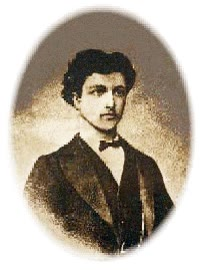
\includegraphics[width=\linewidth]{images/book3/b1-mohorovicic.jpg}

{\scriptsize Andrija Mohorovičić. Domínio público.}
\end{minipage}
\end{history}

\section{Um modelo de referência da Terra}

O mesmo raciocínio, aplicado a milhões de tempos de percurso em todas as distâncias e aos períodos das oscilações livres da Terra (o planeta inteiro soa como um sino depois de um grande terremoto), dá as velocidades em cada profundidade.

\begin{definition}[Modelo de referência da Terra]\label{def:b1:layered-earth:reference-model}
Um \emph{modelo de referência da Terra}\index{modelo de referência da Terra} é uma Terra com simetria esférica, dada pelas velocidades sísmicas $v_P(r)$, $v_S(r)$, pela densidade $\rho(r)$ e, nos modelos mais completos, pela atenuação, como funções só do raio $r$, que se ajustam aos tempos de percurso observados, aos períodos das oscilações livres, à massa da Terra e ao seu momento de inércia. O mais usado é o PREM, o Preliminary Reference Earth Model (1981).
\end{definition}

PREM foi ajustado ao raio \qty{6371}{km}, à massa \qty{5.974e24}{kg} e ao \omterm{def:b1:comparative-planetology:moi}{fator de momento de inércia} $0.3308$ da Terra. Ele divide o planeta em algumas regiões unidas por descontinuidades, e seus perfis (figura abaixo) mostram de imediato as principais camadas.

\begin{definition}[Crosta, manto, núcleo externo, núcleo interno]\label{def:b1:layered-earth:layers}
A \emph{crosta}\index{crosta} é a camada silicática externa acima da \omterm{def:b1:layered-earth:discontinuity}{Moho}. O \emph{manto}\index{manto} é a casca silicática sólida entre a \omterm{def:b1:layered-earth:discontinuity}{Moho} e o \omterm{def:b1:layered-earth:discontinuity}{limite manto--núcleo}, a uma profundidade de cerca de \qty{2891}{km}. O \emph{núcleo externo}\index{núcleo externo} é a casca metálica líquida entre o \omterm{def:b1:layered-earth:discontinuity}{limite manto--núcleo} e o \omterm{def:b1:layered-earth:discontinuity}{limite do núcleo interno}, a cerca de \qty{5150}{km} de profundidade. O \emph{núcleo interno}\index{núcleo interno} é a esfera metálica sólida abaixo dele, de raio de cerca de \qty{1220}{km}.
\end{definition}

\begin{omfigure}
\begin{tikzpicture}
\begin{axis}[omrecord, omdepth, width=0.62\linewidth, height=5.4cm, xmin=0, xmax=14, ymin=0, ymax=6371,
  xlabel={velocidade (\unit{km.s^{-1}}) ou densidade (\unit{g.cm^{-3}})}, ylabel={profundidade (km)},
  ytick={0,1000,...,6000}, tick label style={font=\scriptsize}, label style={font=\small},
  clip=false, legend style={font=\scriptsize, at={(0.02,0.80)}, anchor=north west, draw=none, fill=white}]
\addplot[very thick, blue!70!black] table[x=vp, y=depth] {figdata/out/bachelor-1-prem_profiles-profiles.dat};
\addlegendentry{$v_P$}
\addplot[very thick, red!75!black] table[x=vs, y=depth] {figdata/out/bachelor-1-prem_profiles-profiles.dat};
\addlegendentry{$v_S$}
\addplot[very thick, black!70, densely dashed] table[x=rho, y=depth] {figdata/out/bachelor-1-prem_profiles-profiles.dat};
\addlegendentry{$\rho$}
\draw[black!35] (axis cs:0,670) -- (axis cs:14,670) node[right, font=\scriptsize, black] {670 km};
\draw[black!35] (axis cs:0,2891) -- (axis cs:14,2891) node[right, font=\scriptsize, black] {limite manto--núcleo};
\draw[black!35] (axis cs:0,5149.5) -- (axis cs:14,5149.5) node[right, font=\scriptsize, black] {limite do núcleo interno};
\node[font=\scriptsize, anchor=west] at (axis cs:14,1700) {manto};
\node[font=\scriptsize, anchor=west] at (axis cs:14,4000) {núcleo externo (líquido)};
\node[font=\scriptsize, anchor=west] at (axis cs:14,5800) {núcleo interno (sólido)};
\end{axis}
\end{tikzpicture}

\par\smallskip{\small PREM: as velocidades das ondas P e S e a densidade em função da profundidade. A velocidade S cai a zero no \omterm{def:b1:layered-earth:layers}{núcleo externo} líquido e reaparece, pequena, no \omterm{def:b1:layered-earth:layers}{núcleo interno} sólido; no \omterm{def:b1:layered-earth:discontinuity}{limite manto--núcleo} a densidade quase dobra enquanto $v_P$ cai de 13.7 para \qty{8.1}{km.s^{-1}}; os saltos perto de \qty{400}{km} e \qty{670}{km} delimitam a zona de transição.}
\end{omfigure}

\begin{table}[htbp]
\centering
\footnotesize
\setlength{\tabcolsep}{3pt}
\begin{tabular}{>{\raggedright\arraybackslash}p{0.2\linewidth}rr>{\raggedright\arraybackslash}p{0.47\linewidth}}
\hline
limite no PREM & profundidade (km) & raio (km) & o que muda \\
\hline
\omterm{def:b1:layered-earth:discontinuity}{Moho} & 24.4 & 6346.6 & \omterm{def:b1:layered-earth:layers}{crosta} acima, peridotito abaixo; $v_P$ de 6.8 a 8.1 \\
descontinuidade de 220 km & 220 & 6151 & base da \omterm{def:b1:layered-earth:lithosphere}{zona de baixa velocidade} no PREM \\
descontinuidade de 400 km & 400 & 5971 & \omterm{def:b1:rock-forming-minerals:groups}{olivina} para wadsleíta (\qty{410}{km} na maioria dos estudos) \\
descontinuidade de 670 km & 670 & 5701 & ringwoodita para bridgmanita e ferropericlásio (\qty{660}{km} na maioria dos estudos) \\
\omterm{def:b1:layered-earth:discontinuity}{limite manto--núcleo} & 2891 & 3480 & silicato para ferro líquido; $v_S$ de 7.3 a 0; $\rho$ de 5.57 a 9.90 \\
\omterm{def:b1:layered-earth:discontinuity}{limite do núcleo interno} & 5149.5 & 1221.5 & ferro líquido para sólido; $v_S$ de 0 a 3.5; $\rho$ de 12.17 a 12.76 \\
\hline
\end{tabular}
\caption{As principais descontinuidades do PREM (velocidades em \unit{km.s^{-1}}, densidades em \unit{g.cm^{-3}}). O PREM faz a média da \omterm{def:b1:layered-earth:layers}{crosta} em \qty{24.4}{km}; as \omterm{def:b1:layered-earth:layers}{crostas} reais variam de cerca de \qty{5}{km} sob os oceanos a muitas dezenas de quilômetros sob as cadeias de montanhas.}
% ledger: usgs:crust-thickness
\label{tab:b1:layered-earth:prem}
\end{table}

Dois fatos desses perfis são observados diretamente. A anulação de $v_S$ no \omterm{def:b1:layered-earth:layers}{núcleo externo} é a sombra das ondas S lembrada acima: as ondas S entram no núcleo apenas como ondas P, o núcleo não transmite cisalhamento, logo é líquido. E o \omterm{def:b1:layered-earth:layers}{núcleo interno} transmite ondas S, lentamente: é sólido. Esse segundo fato veio de chegadas P fracas onde nenhuma onda P deveria chegar.

\begin{history}[Inge Lehmann e o núcleo interno]
% ledger: hjortenberg:lehmann
\begin{minipage}[t]{0.76\linewidth}\vspace{0pt}
Inge Lehmann (1888--1993), chefe do departamento de sismologia do instituto geodésico dinamarquês, estudou os registros do terremoto de Buller de 1929, na Nova Zelândia, e encontrou ondas P chegando dentro da zona de sombra, onde o núcleo deveria tê-las desviado. Em um artigo de 1936 com o mais curto dos títulos, \emph{P$'$}, mostrou que elas podiam ser explicadas se o núcleo tivesse um \omterm{def:b1:layered-earth:layers}{núcleo interno} menor, com velocidade P mais alta, que devolve parte da energia para a superfície. Sabe-se hoje que o seu \omterm{def:b1:layered-earth:layers}{núcleo interno} é sólido e cresce lentamente à medida que a Terra esfria. Ela descobriu também a descontinuidade perto de \qty{220}{km} que leva o seu nome.
\end{minipage}\hfill
\begin{minipage}[t]{0.2\linewidth}\vspace{0pt}
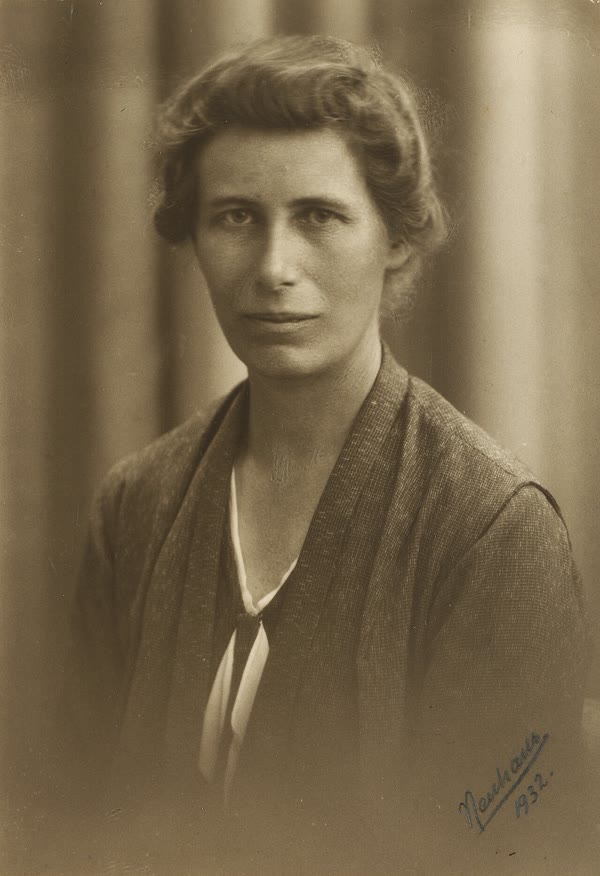
\includegraphics[width=\linewidth]{images/book3/b1-lehmann.jpg}

{\scriptsize Inge Lehmann em 1932, por Even Neuhaus. Domínio público.}
\end{minipage}
\end{history}

\section{Densidade, gravidade e pressão a partir de dados sísmicos}

As velocidades sísmicas dão duas combinações dos módulos e da densidade, não a própria densidade. Uma terceira relação vem da suposição de que, no interior de uma camada de composição uniforme, a rocha é simplesmente comprimida pelo peso da rocha acima.

\begin{definition}[Parâmetro sísmico]\label{def:b1:layered-earth:seismic-parameter}
O \emph{parâmetro sísmico}\index{parâmetro sísmico} em uma profundidade é
\[
  \Phi = v_P^2 - \tfrac43 v_S^2 = \frac{K}{\rho},
\]
o módulo de compressão dividido pela densidade, calculado só a partir das duas velocidades sísmicas (\cref{prop:b1:layered-earth:speeds}).
\end{definition}

\begin{theorem}[Equação de Adams--Williamson]\label{thm:b1:layered-earth:adams-williamson}
Em uma região de composição uniforme, em equilíbrio hidrostático, comprimida adiabaticamente, a densidade varia com o raio como
\[
  \frac{\mathrm d\rho}{\mathrm dr} = -\frac{\rho(r)\,g(r)}{\Phi(r)},
\]
onde $g(r)$ é a gravidade no raio $r$.
\end{theorem}

\begin{proof}
O equilíbrio hidrostático dá $\mathrm dP/\mathrm dr = -\rho g$ (lembrando que $\mathrm dz = -\mathrm dr$). O módulo de compressão é definido por $K = \rho\,\mathrm dP/\mathrm d\rho$ para a compressão em questão; para uma rocha de composição fixa comprimida sem troca de calor, é o módulo adiabático que as ondas sísmicas medem, de modo que $\mathrm d\rho/\mathrm dP = \rho/K$. Pela regra da cadeia,
\[
  \frac{\mathrm d\rho}{\mathrm dr} = \frac{\mathrm d\rho}{\mathrm dP}\,
  \frac{\mathrm dP}{\mathrm dr} = \frac{\rho}{K}\,(-\rho g) = -\frac{\rho g}{K/\rho}
  = -\frac{\rho g}{\Phi}. \qedhere
\]
\end{proof}

A equação falha em uma descontinuidade, onde a composição ou a estrutura cristalina muda, e onde quer que a temperatura se afaste do adiabático; mas entre as descontinuidades ela explica muito bem o aumento observado da densidade com a profundidade (painel (c) da figura abaixo). Partindo de uma densidade no topo de cada região, integrando-a para baixo e ajustando os valores iniciais até que a massa e o momento de inércia saiam corretos, foi assim que os primeiros modelos de densidade foram construídos. Os dois números globais são integrais da densidade.

\begin{proposition}[Massa, gravidade, pressão e momento de inércia]
\label{prop:b1:layered-earth:integrals}
Para uma Terra de simetria esférica de raio $R$ e densidade $\rho(r)$, a massa dentro do raio $r$, a gravidade, a pressão e o momento de inércia em torno de um eixo pelo centro são
\[
  m(r) = \int_0^r 4\pi s^2\rho(s)\,\mathrm ds, \quad
  g(r) = \frac{G\,m(r)}{r^2}, \quad
  P(r) = \int_r^R \rho(s)\,g(s)\,\mathrm ds, \quad
  I = \frac{8\pi}{3}\int_0^R \rho(r)\,r^4\,\mathrm dr.
\]
\end{proposition}

\begin{proof}
Uma casca fina de raio $s$ e espessura $\mathrm ds$ tem o volume $4\pi s^2\,\mathrm ds$, daí a primeira integral. A gravidade de um corpo de simetria esférica fora de um raio é a de sua massa interior, concentrada no centro, e as cascas exteriores a $r$ puxam sem força resultante (o teorema da casca,
  que os livros de física demonstram); daí $g(r)$. Integrando a equação hidrostática a partir da superfície, onde $P = 0$, obtém-se $P(r)$. Para o momento de inércia, uma casca esférica fina de massa $\mathrm dm$ e raio $r$ tem, em torno dos três eixos $x$, $y$, $z$, momentos cuja soma é
$\int (y^2 + z^2) + (z^2 + x^2) + (x^2 + y^2)\,\mathrm dm = 2r^2\,\mathrm dm$;
por simetria os três são iguais, logo cada um é $\tfrac23 r^2\,\mathrm dm$. Com $\mathrm dm = 4\pi r^2\rho\,\mathrm dr$, somando as cascas obtém-se $I$.
\end{proof}

Para uma esfera de densidade uniforme, $I = \tfrac{8\pi}{15}\rho R^5 = 0.4\,MR^2$.
O fator $I/MR^2 = 0.3308$ da Terra é menor: sua massa se concentra em direção ao centro, que é o primeiro argumento para um núcleo denso. Calculadas só a partir da densidade do PREM, as integrais dão uma massa de \qty{5.976e24}{kg} (\qty{0.06}{\percent} acima da medida \qty{5.972e24}{kg}), um fator $0.3309$, e uma pressão central de \qty{364}{GPa}, o valor tabelado com o PREM a \qty{0.1}{\percent}.

\begin{omfigure}
\begin{tabular}{@{}c@{\hspace{2mm}}c@{\hspace{2mm}}c@{}}
\begin{tikzpicture}
\begin{axis}[omrecord, omdepth, width=0.35\linewidth, height=7.0cm, xmin=0, xmax=12, ymin=0, ymax=6371,
  xlabel={$g$ (\unit{m.s^{-2}})}, ylabel={profundidade (km)}, ytick={0,1000,...,6000}, xtick={0,4,8,12},
  tick label style={font=\scriptsize}, label style={font=\small}]
\addplot[very thick, blue!70!black] table[x=g, y=depth] {figdata/out/bachelor-1-prem_profiles-functionals.dat};
\draw[black!35] (axis cs:0,2891) -- (axis cs:12,2891);
\draw[black!35] (axis cs:0,5149.5) -- (axis cs:12,5149.5);
\node[font=\scriptsize, anchor=south west] at (axis cs:0.3,2891) {CMB};
\node[font=\scriptsize, anchor=south west] at (axis cs:0.3,5149.5) {ICB};
\end{axis}
\end{tikzpicture}
&
\begin{tikzpicture}
\begin{axis}[omrecord, omdepth, width=0.35\linewidth, height=7.0cm, xmin=0, xmax=400, ymin=0, ymax=6371,
  xlabel={$P$ (GPa)}, ytick={0,1000,...,6000}, yticklabels={}, xtick={0,200,400},
  tick label style={font=\scriptsize}, label style={font=\small}]
\addplot[very thick, red!75!black] table[x=P, y=depth] {figdata/out/bachelor-1-prem_profiles-functionals.dat};
\draw[black!35] (axis cs:0,2891) -- (axis cs:400,2891);
\draw[black!35] (axis cs:0,5149.5) -- (axis cs:400,5149.5);
\node[font=\scriptsize, anchor=south west] at (axis cs:150,2891) {\qty{136}{GPa}};
\node[font=\scriptsize, anchor=south east] at (axis cs:290,5149.5) {\qty{329}{GPa}};
\end{axis}
\end{tikzpicture}
&
\begin{tikzpicture}
\begin{axis}[omrecord, omdepth, width=0.35\linewidth, height=7.0cm, xmin=2, xmax=14, ymin=0, ymax=6371,
  xlabel={$\rho$ (\unit{g.cm^{-3}})}, ytick={0,1000,...,6000}, yticklabels={}, xtick={2,6,10,14},
  tick label style={font=\scriptsize}, label style={font=\small},
  legend style={font=\scriptsize, at={(0.97,0.97)}, anchor=north east, draw=none, fill=white}]
\addplot[very thick, black!55] table[x=rho, y=depth] {figdata/out/bachelor-1-prem_profiles-profiles.dat};
\addlegendentry{PREM}
\addplot[only marks, mark=o, mark size=1.4pt, orange!85!black, each nth point=15, unbounded coords=discard]
  table[x=rho_aw, y=depth] {figdata/out/bachelor-1-prem_profiles-adams.dat};
\addlegendentry{Adams--Williamson}
\end{axis}
\end{tikzpicture}
\\[2pt]
{\small (a) gravidade} & {\small (b) pressão} & {\small (c) autocompressão} \\
\end{tabular}

\par\smallskip{\small No interior da Terra, a partir do PREM. (a) e (b) Gravidade e pressão calculadas a partir da densidade do PREM com \cref{prop:b1:layered-earth:integrals}: a gravidade se mantém perto de \qty{10}{m.s^{-2}} através do \omterm{def:b1:layered-earth:layers}{manto}, atinge um máximo de \qty{10.7}{m.s^{-2}} no \omterm{def:b1:layered-earth:discontinuity}{limite manto--núcleo} (CMB) e cai a zero no centro; a pressão chega a \qty{136}{GPa} no CMB, \qty{329}{GPa} no \omterm{def:b1:layered-earth:discontinuity}{limite do núcleo interno} (ICB) e \qty{364}{GPa} no centro. (c) A equação de Adams--Williamson, integrada para baixo a partir da densidade do PREM a \qty{771}{km} e no topo do \omterm{def:b1:layered-earth:layers}{núcleo externo} com as velocidades e a gravidade do PREM (círculos), segue o PREM com \qty{0.2}{\percent}: ali o aumento da densidade é a compressão de um material uniforme; os saltos, não.}
\end{omfigure}

Que a gravidade cresça na descida pelo \omterm{def:b1:layered-earth:layers}{manto} é consequência direta do núcleo denso: a massa deixada dentro do raio cai mais devagar que $r^2$. Através do \omterm{def:b1:layered-earth:layers}{manto} $g$ quase não muda, e a pressão cresce quase linearmente com a profundidade, cerca de \qty{4.7}{GPa} por cem quilômetros.


\section{O manto: uma rocha, várias associações minerais}

O \omterm{def:b1:layered-earth:layers}{manto} superior é peridotito, conhecido pelos fragmentos que os vulcões trazem à superfície e por fatias do \omterm{def:b1:layered-earth:layers}{manto} empurradas sobre os continentes: cerca de metade a três quintos de \omterm{def:b1:rock-forming-minerals:groups}{olivina} em volume (\qtyrange{49}{62}{\percent} nas composições propostas), o resto \omterm{def:b1:rock-forming-minerals:groups}{piroxênios} e um \omterm{def:b1:rock-forming-minerals:mineral}{mineral} alumínico (\omterm{def:b1:rock-forming-minerals:groups}{plagioclásio}, espinélio ou \omterm{def:b1:rock-forming-minerals:groups}{granada}, conforme a profundidade). A pressão que cresce com a profundidade não muda essa composição, mas força os seus átomos em arranjos mais densos: \omterm{def:b1:rock-forming-minerals:polymorph}{polimorfos} (\cref{ch:b1:rock-forming-minerals}) aparecem um após o outro.

\begin{definition}[Zona de transição do manto]\label{def:b1:layered-earth:transition-zone}
A \emph{zona de transição do manto}\index{zona de transição do manto} é a parte do \omterm{def:b1:layered-earth:layers}{manto} entre as \omterm{def:b1:layered-earth:discontinuity}{descontinuidades sísmicas} perto de \qty{410}{km} e \qty{660}{km} de profundidade, em que a \omterm{def:b1:rock-forming-minerals:groups}{olivina} do \omterm{def:b1:layered-earth:layers}{manto} superior é substituída pelos seus \omterm{def:b1:rock-forming-minerals:polymorph}{polimorfos} mais densos, a wadsleíta e depois a ringwoodita. Acima dela fica o \omterm{def:b1:layered-earth:layers}{manto} superior; abaixo, o \omterm{def:b1:layered-earth:layers}{manto} inferior, até o \omterm{def:b1:layered-earth:discontinuity}{limite manto--núcleo}.
\end{definition}

Em cerca de \qty{410}{km} (\qty{14}{GPa}) a \omterm{def:b1:rock-forming-minerals:groups}{olivina} \ce{(Mg,Fe)2SiO4} se torna wadsleíta, de mesma fórmula; perto de \qty{520}{km} (\qty{17.5}{GPa}) a wadsleíta se torna ringwoodita; os \omterm{def:b1:rock-forming-minerals:groups}{piroxênios} se dissolvem em uma \omterm{def:b1:rock-forming-minerals:groups}{granada} rica em silício, a majorita, até que, no meio da zona de transição, a \omterm{def:b1:rock-forming-minerals:groups}{granada} contém todos eles, de modo que a zona é um pouco mais que metade de \omterm{def:b1:rock-forming-minerals:polymorph}{polimorfos} da \omterm{def:b1:rock-forming-minerals:groups}{olivina} e o resto \omterm{def:b1:rock-forming-minerals:groups}{granada}. Em cerca de \qty{660}{km}, a uma pressão perto de \qty{24}{GPa}, a ringwoodita se decompõe em
dois \omterm{def:b1:rock-forming-minerals:mineral}{minerais}, escritos para o \omterm{def:b1:rock-forming-minerals:solid-solution}{membro-final} magnesiano
\[
  \ce{Mg2SiO4 -> MgSiO3 + MgO}:
\]
bridgmanita, \ce{(Mg,Fe)SiO3} com a estrutura da perovskita, e ferropericlásio, \ce{(Mg,Fe)O}. Um \omterm{def:b1:layered-earth:layers}{manto} inferior de mesma composição que o \omterm{def:b1:layered-earth:layers}{manto} superior é cerca de \qty{75}{\percent} bridgmanita, \qty{17}{\percent} ferropericlásio e \qty{8}{\percent} de uma perovskita silicática de cálcio, em volume, e se ajusta às densidades e velocidades do \omterm{def:b1:layered-earth:reference-model}{modelo de referência}. A bridgmanita é, portanto, o \omterm{def:b1:rock-forming-minerals:mineral}{mineral} mais abundante da Terra; ela recebeu o seu nome só em 2014, depois que grãos naturais foram descritos em um meteorito fortemente chocado.
% ledger: frost:mantle-transitions, sun:lower-mantle, tschauner:bridgmanite

Cada mudança produz \omterm{def:b1:rock-forming-minerals:mineral}{minerais} mais densos, de modo que aumenta a densidade e as velocidades sísmicas: as transições são as descontinuidades dos perfis (figura abaixo). Suas profundidades não são fixas. Uma mudança de fase ocorre a uma pressão que depende da temperatura, e a inclinação dessa dependência (a inclinação de Clapeyron, tratada no Livro 4) faz a descontinuidade de \qty{410}{km} subir e a de \qty{660}{km} descer na rocha fria de uma placa que afunda. Mapear a topografia das descontinuidades é uma maneira de encontrar regiões frias e quentes no \omterm{def:b1:layered-earth:layers}{manto}.

\begin{omfigure}
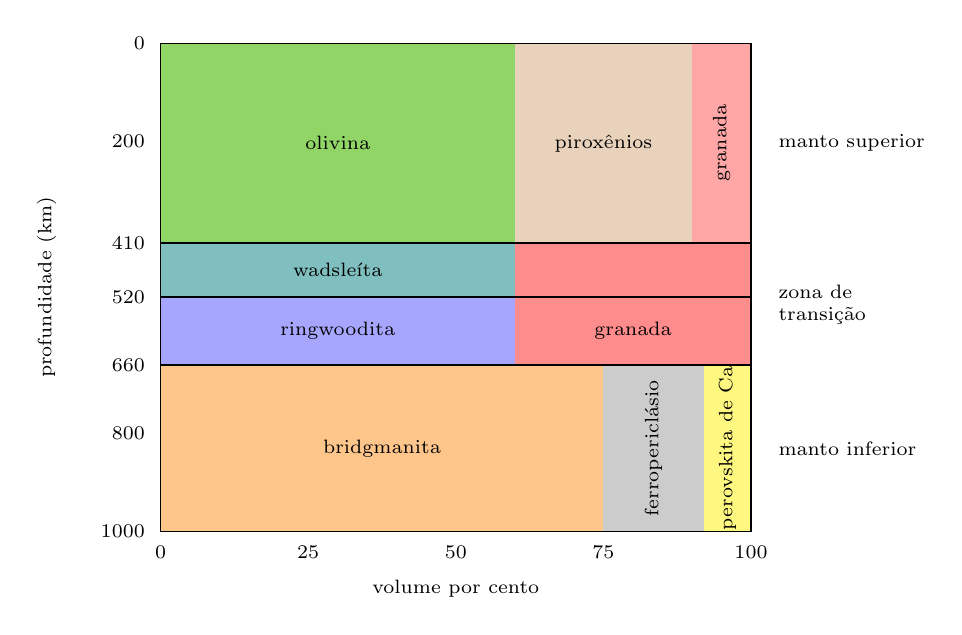
\begin{tikzpicture}[x=0.075mm, y=-0.062mm, font=\scriptsize]
% schematic volume fractions (ledger frost:mantle-transitions, sun:lower-mantle)
\def\W{1000}
% upper mantle 0-410: olivine 60, pyroxenes 30, garnet 10
\fill[green!45!olive!60] (0,0) rectangle (600,410);
\fill[brown!35] (600,0) rectangle (900,410);
\fill[red!35] (900,0) rectangle (1000,410);
% 410-520 wadsleyite 60, garnet 40 ; 520-660 ringwoodite 60, garnet 40
\fill[teal!50] (0,410) rectangle (600,520);
\fill[blue!35] (0,520) rectangle (600,660);
\fill[red!45] (600,410) rectangle (1000,660);
% 660-1000 bridgmanite 75, ferropericlase 17, Ca-perovskite 8
\fill[orange!45] (0,660) rectangle (750,1000);
\fill[gray!40] (750,660) rectangle (920,1000);
\fill[yellow!50] (920,660) rectangle (1000,1000);
\draw (0,0) rectangle (1000,1000);
\foreach \d in {410,520,660} \draw[thick] (0,\d) -- (1000,\d);
\node at (300,205) {olivina};
\node[align=center] at (750,205) {piroxênios};
\node[rotate=90] at (950,205) {granada};
\node at (300,465) {wadsleíta};
\node at (300,590) {ringwoodita};
\node[align=center] at (800,590) {granada};
\node at (375,830) {bridgmanita};
\node[rotate=90, align=center] at (835,830) {ferropericlásio};
\node[rotate=90] at (960,830) {perovskita de Ca};
\foreach \d in {0,200,410,520,660,800,1000} \node[anchor=east] at (-10,\d) {\d};
\node[rotate=90, anchor=south] at (-160,500) {profundidade (km)};
\foreach \p in {0,25,50,75,100} \node[anchor=north] at (\p*10,1010) {\p};
\node[anchor=north] at (500,1080) {volume por cento};
\node[anchor=west, align=left] at (1030,205) {manto superior};
\node[anchor=west, align=left] at (1030,535) {zona de\\transição};
\node[anchor=west, align=left] at (1030,830) {manto inferior};
\end{tikzpicture}

\par\smallskip{\small Os \omterm{def:b1:rock-forming-minerals:mineral}{minerais} de um \omterm{def:b1:layered-earth:layers}{manto} de peridotito com a profundidade, como frações de volume (esquemático: as fronteiras são traçadas nítidas, e as frações são valores redondos dentro das faixas citadas no texto). A composição não muda; os \omterm{def:b1:rock-forming-minerals:mineral}{minerais} mudam, a cerca de 410, 520 e \qty{660}{km}.}
\end{omfigure}

Na base do \omterm{def:b1:layered-earth:layers}{manto}, a camada chamada D$''$ (D duas linhas, nome mantido de um modelo antigo da Terra) tem um gradiente de velocidade diferente do resto do \omterm{def:b1:layered-earth:layers}{manto} inferior; o PREM lhe atribui os \qty{150}{km} mais baixos do \omterm{def:b1:layered-earth:layers}{manto}. É heterogênea sismicamente: manchas de velocidade muito baixa, gradientes íngremes, refletores. Pensa-se que seja uma camada limite entre o núcleo quente e o \omterm{def:b1:layered-earth:layers}{manto}, e talvez um cemitério de placas antigas.
% ledger: prem:dpp

\section{O núcleo}

O núcleo é sobretudo ferro. Sua densidade, suas velocidades e sua capacidade de gerar um campo magnético apontam para um metal, e o ferro é de longe o elemento mais abundante entre os suficientemente densos que os meteoritos e o Sol mostram ser comuns. O níquel, abundante nos meteoritos de ferro, o acompanha. Mas o núcleo não é ferro--níquel puro.
\begin{itemize}
  \item O núcleo é \qtyrange{5}{10}{\percent} menos denso do que o ferro puro seria nas mesmas pressão e temperatura: deve conter elementos leves, entre os quais silício, enxofre, carbono, oxigênio e hidrogênio são os candidatos.
  \item A densidade salta cerca de \qty{4.5}{\percent} no \omterm{def:b1:layered-earth:discontinuity}{limite do núcleo interno}, muito para o congelamento de um só e mesmo metal: o \omterm{def:b1:layered-earth:layers}{núcleo interno} também contém elementos leves, mas menos, alguns por cento, contra \qtyrange{5}{10}{\percent} no líquido.
\end{itemize}
% ledger: badro:core
A diferença tem uma consequência. À medida que a Terra esfria --- seu \omterm{def:b1:layered-earth:layers}{manto} cerca de \qty{100}{\degreeCelsius} por bilhão de anos atualmente ---, o líquido do núcleo congela sobre o \omterm{def:b1:layered-earth:layers}{núcleo interno}, que cresce, e
% ledger: bellini:cooling
o congelamento deixa a maior parte dos elementos leves no líquido. O líquido leve liberado na base do \omterm{def:b1:layered-earth:layers}{núcleo externo} sobe, e acredita-se que essa flutuabilidade ajude a agitar o \omterm{def:b1:layered-earth:layers}{núcleo externo} e a acionar o dínamo que gera o campo magnético da Terra.

\section{Camadas mecânicas: litosfera e astenosfera}

As camadas acima são definidas pela composição e pela fase: \omterm{def:b1:layered-earth:layers}{crosta} e \omterm{def:b1:layered-earth:layers}{manto} são rochas diferentes, \omterm{def:b1:layered-earth:layers}{núcleos externo} e interno são estados diferentes. A tectônica de placas precisa de outra divisão, pela resistência, que corta a primeira.

\begin{definition}[Litosfera, astenosfera, zona de baixa velocidade]
\label{def:b1:layered-earth:lithosphere}
A \emph{litosfera}\index{litosfera} é a casca externa rígida da Terra, a \omterm{def:b1:layered-earth:layers}{crosta} e o \omterm{def:b1:layered-earth:layers}{manto} mais superior, que se comporta como uma camada forte ao longo dos tempos geológicos e é dividida em placas. A \emph{astenosfera}\index{astenosfera} é a camada mais fraca do \omterm{def:b1:layered-earth:layers}{manto} superior abaixo dela, que se deforma por um fluxo lento e deixa as placas se moverem. A \emph{zona de baixa velocidade}\index{zona de baixa velocidade} é a faixa de profundidade abaixo da litosfera em que as velocidades sísmicas, sobretudo as das ondas S, são mais baixas do que logo acima e abaixo.
\end{definition}

A \omterm{def:b1:layered-earth:lithosphere}{litosfera} não é uma rocha, e sim uma faixa de temperatura: o peridotito do \omterm{def:b1:layered-earth:layers}{manto} é forte onde está frio e flui onde está quente, e a sua base é aproximadamente uma isoterma. Ela é fina sob as cristas, onde o \omterm{def:b1:layered-earth:layers}{manto} quente sobe, cerca de \qty{140}{km} de espessura sob o assoalho oceânico mais antigo, e \qtyrange{40}{280}{km} de espessura sob os continentes, mais espessa sob os crátons antigos; o topo da \omterm{def:b1:layered-earth:lithosphere}{astenosfera} fica a cerca de \qtyrange{80}{200}{km}. Sismicamente, a \omterm{def:b1:layered-earth:lithosphere}{astenosfera} aparece como a \omterm{def:b1:layered-earth:lithosphere}{zona de baixa velocidade}, perto das suas condições de fusão: no PREM a velocidade S diminui levemente desde a \omterm{def:b1:layered-earth:discontinuity}{Moho} até \qty{220}{km}, onde volta a saltar. Como a resistência depende da temperatura, e por que isso acontece, é o assunto de \cref{ch:b1:stress-strain-rheology}.

\begin{inthefield}[Uma estação sísmica]
\begin{minipage}[t]{0.55\linewidth}\vspace{0pt}
Os tempos de percurso em que se apoiam os \omterm{def:b1:layered-earth:reference-model}{modelos de referência} vêm de estações permanentes. Um sismômetro de banda larga, que registra movimentos do solo de centésimos de segundo a horas de período, fica sobre um pilar de concreto assentado em rocha nua e isolado do piso da cúpula, sob uma cobertura que mantém a sua temperatura estável: uma variação de uma fração de grau, uma corrente de ar ou um caminhão passando apareceria no registro. O registrador de dados marca cada amostra com a hora dada por satélites, e os registros fluem para centros de dados que os compartilham abertamente. Redes dessas estações localizam e datam todos os grandes terremotos; os tempos de chegada lidos em seus registros foram invertidos para obter as velocidades em cada profundidade.
\end{minipage}\hfill
\begin{minipage}[t]{0.42\linewidth}\vspace{0pt}
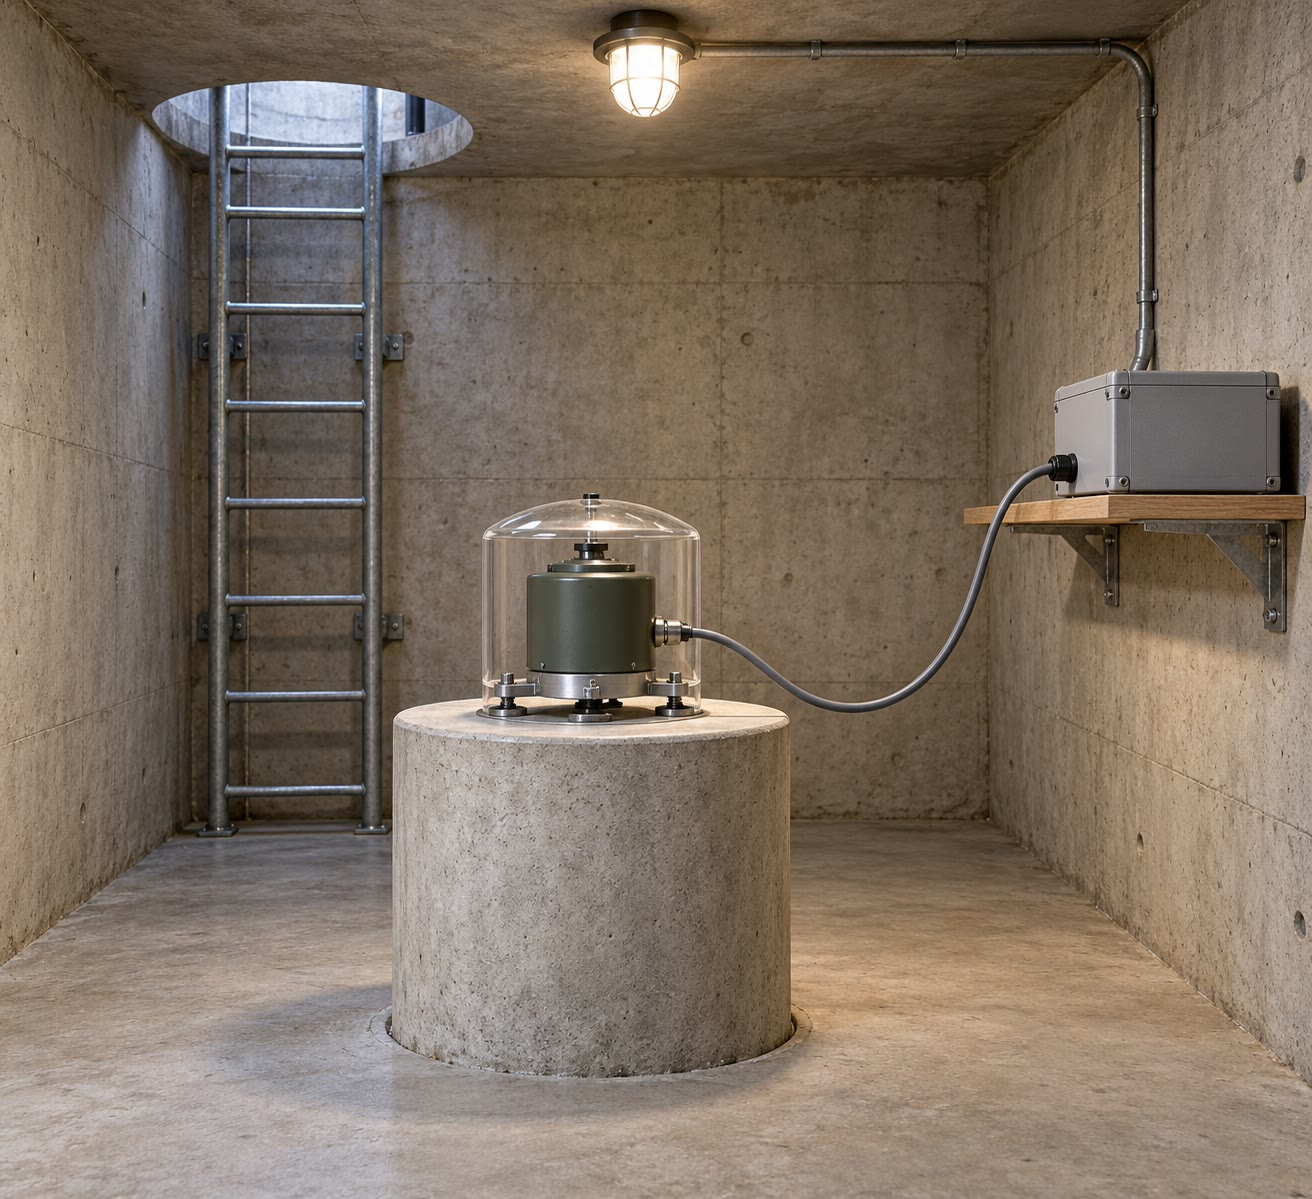
\includegraphics[width=\linewidth]{images/book3/ai/b1-seismometer-vault.jpg}

{\scriptsize Um sismômetro de banda larga sobre o seu pilar em uma cúpula subterrânea, com o registrador de dados na parede (ilustração gerada por IA).}
\end{minipage}
\end{inthefield}

\section{Exercícios}

\begin{exercise}[$\star$]\label{exo:b1:layered-earth:1}
Com os raios do PREM $R = \qty{6371}{km}$, $r_{\text{CMB}} = \qty{3480}{km}$ e $r_{\text{ICB}} = \qty{1221.5}{km}$, calcule as frações do volume da Terra ocupadas pelo núcleo e pelo \omterm{def:b1:layered-earth:layers}{núcleo interno}.
% ledger: prem:cmb, prem:icb
\end{exercise}

\begin{exercise}[$\star$]\label{exo:b1:layered-earth:2}
Logo acima do \omterm{def:b1:layered-earth:discontinuity}{limite manto--núcleo} o PREM dá $v_P = \qty{13.7166}{km.s^{-1}}$,
$v_S = \qty{7.26466}{km.s^{-1}}$, $\rho = \qty{5.56645}{g.cm^{-3}}$; logo abaixo,
$v_P = \qty{8.06482}{km.s^{-1}}$, $v_S = 0$, $\rho = \qty{9.90349}{g.cm^{-3}}$.
Calcule o \omterm{def:b1:layered-earth:seismic-parameter}{parâmetro sísmico} e o módulo de compressão de cada lado (em GPa). O que muda mais através do limite?
% ledger: data:prem, prem:cmb
\end{exercise}

\begin{exercise}[$\star$]\label{exo:b1:layered-earth:3}
Uma \omterm{def:b1:layered-earth:layers}{crosta} de \qty{30}{km} de espessura, a \qty{6.2}{km.s^{-1}}, repousa sobre um \omterm{def:b1:layered-earth:layers}{manto} a
\qty{8.1}{km.s^{-1}}. Calcule o ângulo crítico, a distância crítica e a \omterm{def:b1:layered-earth:head-wave}{distância de cruzamento}.
\end{exercise}

\begin{exercise}[$\star$]\label{exo:b1:layered-earth:4}
A massa do núcleo é \qty{1.94e24}{kg} e o seu raio \qty{3480}{km}. Calcule a gravidade no \omterm{def:b1:layered-earth:discontinuity}{limite manto--núcleo} e compare-a com a gravidade na superfície, \qty{9.82}{m.s^{-2}}. Por que ela é maior?
\end{exercise}

\begin{exercise}[$\star\star$]\label{exo:b1:layered-earth:5}
Em um perfil de refração as primeiras chegadas estão em \qty{10.0}{s} a \qty{60}{km}, em \qty{33.3}{s} a \qty{200}{km} e em \qty{45.8}{s} a \qty{300}{km}; a reta pelo primeiro ponto passa pela origem. Encontre $v_1$, $v_2$, o tempo de interseção e a profundidade da fronteira, e confira o resultado com a \omterm{def:b1:layered-earth:head-wave}{distância de cruzamento}.
\end{exercise}

\begin{exercise}[$\star\star$]\label{exo:b1:layered-earth:6}
Mostre que uma esfera homogênea tem $I = 0.4\,MR^2$. Depois calcule a massa e o fator $I/MR^2$ de uma Terra de duas camadas: um núcleo de raio \qty{3480}{km} e densidade \qty{11.0}{g.cm^{-3}} em um \omterm{def:b1:layered-earth:layers}{manto} de densidade \qty{4.45}{g.cm^{-3}}, com $R = \qty{6371}{km}$. Compare com \num{5.972e24} kg e $0.3308$.
\end{exercise}

\begin{exercise}[$\star\star$]\label{exo:b1:layered-earth:7}
Em \qty{1471}{km} de profundidade o PREM dá $v_P = \qty{12.16}{km.s^{-1}}$,
$v_S = \qty{6.673}{km.s^{-1}}$, $\rho = \qty{4.86}{g.cm^{-3}}$, e a gravidade é \qty{9.9}{m.s^{-2}}. Calcule o gradiente de densidade dado pela equação de Adams--Williamson, em \unit{g.cm^{-3}} por \qty{1000}{km}, e compare com as densidades do PREM, \num{4.844} a \qty{1471}{km} e \num{5.357} a \qty{2471}{km}.
% ledger: data:prem
\end{exercise}

\begin{exercise}[$\star\star$]\label{exo:b1:layered-earth:8}
Estime a pressão a \qty{670}{km} de profundidade a partir de uma densidade média de \qty{3.57}{g.cm^{-3}} e uma gravidade de \qty{9.9}{m.s^{-2}}. Que mudança \omterm{def:b1:rock-forming-minerals:mineral}{mineral} é esperada ali?
% ledger: frost:mantle-transitions
\end{exercise}

\begin{exercise}[$\star\star$]\label{exo:b1:layered-earth:9}
A densidade média do \omterm{def:b1:layered-earth:layers}{núcleo externo} do PREM é \qty{10.90}{g.cm^{-3}}; no \omterm{def:b1:layered-earth:discontinuity}{limite do núcleo interno} sua densidade é \qty{12.166}{g.cm^{-3}} acima e \qty{12.764}{g.cm^{-3}} abaixo. (a)~Se o ferro nas mesmas condições é \qtyrange{5}{10}{\percent} mais denso que o \omterm{def:b1:layered-earth:layers}{núcleo externo}, que faixa de densidades isso dá para o ferro líquido ali? (b)~Calcule o salto de densidade no \omterm{def:b1:layered-earth:discontinuity}{limite do núcleo interno} em porcentagem, e compare-o com os \qty{4.5}{\percent} de estudos recentes. (c)~O que um salto maior do que o da solidificação sozinha daria a dizer sobre os elementos leves?
% ledger: badro:core, prem:icb
\end{exercise}

\begin{exercise}[$\star\star\star$]\label{exo:b1:layered-earth:10}
Mostre que o tempo da onda refletida $t_r(x) = \sqrt{x^2 + 4h^2}/v_1$ e o tempo da \omterm{def:b1:layered-earth:head-wave}{onda de cabeça} de \cref{thm:b1:layered-earth:two-layer} são iguais, e têm inclinações iguais, em $x = 2h\tan i_c$, e que $t_r > t_{\text{cabeça}}$ além dela. Interprete.
\end{exercise}

\begin{exercise}[$\star\star\star$]\label{exo:b1:layered-earth:11}
Para uma Terra de densidade uniforme $\rho$, mostre que $g(r) = \tfrac43\pi G\rho r$
e $P(r) = \tfrac23\pi G\rho^2(R^2 - r^2)$. Calcule a pressão central com $\rho = \qty{5513}{kg.m^{-3}}$ e $R = \qty{6371}{km}$, e compare com os \qty{363.85}{GPa} do PREM.
% ledger: earth:density, prem:centre
\end{exercise}

\begin{exercise}[$\star\star\star$]\label{exo:b1:layered-earth:12}
Mostre que, se $g/\Phi$ é constante através de uma camada, a equação de Adams--Williamson dá $\rho = \rho_0\exp\bigl(g(z - z_0)/\Phi\bigr)$ com a profundidade $z$. Aplique-a ao \omterm{def:b1:layered-earth:layers}{núcleo externo}, de \qty{2891}{km} ($\rho_0 =
\qty{9.90}{g.cm^{-3}}$) a \qty{5149.5}{km}, com valores médios
$g = \qty{7.9}{m.s^{-2}}$ e $\Phi = \qty{87}{km^2.s^{-2}}$; compare com os \qty{12.17}{g.cm^{-3}} do PREM no \omterm{def:b1:layered-earth:discontinuity}{limite do núcleo interno}.
% ledger: prem:icb
\end{exercise}

\section{Problema: pesando as cascas da Terra}

\begin{problem}[{Problema de fim de semana --- volumes, massas e momento de inércia de uma Terra de quatro cascas construída a partir do PREM, comparados com a massa e o momento de inércia medidos; gravidade e pressão no fundo do interior}]
\label{pb:b1:layered-earth:1}
% values: calc/ch09.py; mean densities rounded from figdata prem_profiles (values part)
% ledger: data:prem, prem:constraints, prem:centre, prem:cmb, earth:mass, earth:MoI, const:G
A Terra é cortada em quatro cascas nos raios do PREM, e cada uma recebe a sua densidade média no PREM, arredondada:
\begin{center}
\small
\begin{tabular}{lccc}
\hline
casca & de (km) & até (km) & densidade média (\unit{g.cm^{-3}}) \\
\hline
\omterm{def:b1:layered-earth:layers}{crosta}, \omterm{def:b1:layered-earth:layers}{manto} superior e zona de transição & 5701 & 6371 & 3.57 \\
\omterm{def:b1:layered-earth:layers}{manto} inferior & 3480 & 5701 & 4.90 \\
\omterm{def:b1:layered-earth:layers}{núcleo externo} & 1221.5 & 3480 & 10.90 \\
\omterm{def:b1:layered-earth:layers}{núcleo interno} & 0 & 1221.5 & 12.89 \\
\hline
\end{tabular}
\end{center}
Use $G = \qty{6.674e-11}{m^3.kg^{-1}.s^{-2}}$. A massa medida da Terra é \qty{5.972e24}{kg} e o seu \omterm{def:b1:comparative-planetology:moi}{fator de momento de inércia} $I/MR^2 = 0.3308$.

\medskip
\noindent\textbf{Parte I --- Volumes.}
\begin{enumerate}
  \item Calcule o volume da Terra.
  \item Calcule o volume de cada casca.
  \item Que fração do volume ocupa cada casca? Qual é a maior?
  \item Que fração do volume é núcleo?
\end{enumerate}

\noindent\textbf{Parte II --- Massas.}
\begin{enumerate}[resume]
  \item Calcule a massa de cada casca.
  \item Some-as, e compare o total com a massa medida.
  \item Deduza a densidade média da Terra modelo.
  \item Que fração da massa está no \omterm{def:b1:layered-earth:layers}{núcleo interno}?
  \item Que fração da massa está no \omterm{def:b1:layered-earth:layers}{manto} e na \omterm{def:b1:layered-earth:layers}{crosta} juntos?
  \item Compare a parcela do núcleo no volume e na massa, e explique.
\end{enumerate}

\noindent\textbf{Parte III --- Momento de inércia.}
\begin{enumerate}[resume]
  \item Mostre a partir de \cref{prop:b1:layered-earth:integrals} que uma casca homogênea entre $r_1$ e $r_2$ tem $I = \tfrac{8\pi}{15}\rho\,(r_2^5 - r_1^5)$.
  \item Calcule o momento de inércia de cada casca.
  \item Qual casca contribui mais, e por que o \omterm{def:b1:layered-earth:layers}{núcleo interno} contribui quase nada?
  \item Some-os e calcule $I/MR^2$ para o modelo.
  \item Compare com $0.3308$ e com os $0.4$ de uma esfera homogênea.
  \item Dentro de cada casca real a densidade cresce com a profundidade. Isso explica por que o fator do modelo é alto demais? Explique.
\end{enumerate}

\noindent\textbf{Parte IV --- Gravidade e pressão.}
\begin{enumerate}[resume]
  \item Calcule a gravidade na superfície do modelo.
  \item Calcule a gravidade no \omterm{def:b1:layered-earth:discontinuity}{limite manto--núcleo}.
  \item Calcule a densidade média do \omterm{def:b1:layered-earth:layers}{manto} e da \omterm{def:b1:layered-earth:layers}{crosta} juntos.
  \item A gravidade no \omterm{def:b1:layered-earth:layers}{manto} se mantém perto de \qty{10}{m.s^{-2}}. Estime a pressão no \omterm{def:b1:layered-earth:discontinuity}{limite manto--núcleo}, e compare com os \qty{135.75}{GPa} do PREM.
  \item Calcule a densidade média do núcleo, e o aumento de pressão do \omterm{def:b1:layered-earth:discontinuity}{limite manto--núcleo} até o centro em um núcleo homogêneo, $\tfrac23\pi G\rho_c^2 r_c^2$ (\cref{exo:b1:layered-earth:11} aplicado só ao núcleo).
  \item Some as duas para estimar a pressão central, e compare com os \qty{363.85}{GPa} do PREM. Por que a estimativa é baixa demais?
  \item Quais números do modelo são conferidos com uma medida, e quais só com o próprio PREM?
  \item Que fração da massa da Terra está no núcleo?
\end{enumerate}
\end{problem}
